\documentclass[10pt, conference]{IEEEtran}

% Packages
\usepackage{amsmath, amssymb, amsthm}
\usepackage{bm}
\usepackage{graphicx}
\usepackage{subcaption}
\usepackage{algorithm}
\usepackage{algorithmic}
\usepackage{cite}
\usepackage{hyperref}
% Add missing packages for tables, tikz, appendix
\usepackage{booktabs}
\usepackage{multirow}
\usepackage{tikz}
\usetikzlibrary{positioning}

% Theorem environments
\newtheorem{theorem}{Theorem}
\newtheorem{lemma}{Lemma}
\newtheorem{proposition}{Proposition}
\newtheorem{corollary}{Corollary}
\newtheorem{definition}{Definition}
\newtheorem{assumption}{Assumption}
\newtheorem{remark}{Remark}

% Custom commands
\newcommand{\Real}{\mathbb{R}}
\newcommand{\Natural}{\mathbb{N}}
\newcommand{\Expect}{\mathbb{E}}
\newcommand{\Prob}{\mathbb{P}}
\newcommand{\KL}[2]{\mathrm{KL}\left(#1 \parallel #2\right)}
\newcommand{\Normal}{\mathcal{N}}
\newcommand{\Uniform}{\mathcal{U}}
\newcommand{\Laplace}{\mathcal{L}}
\newcommand{\Bernoulli}{\mathrm{Bernoulli}}
\newcommand{\given}{\,|\,}
\newcommand{\argmax}{\operatorname*{arg\,max}}
\newcommand{\argmin}{\operatorname*{arg\,min}}

% Title and author
\title{Conditional Variational Autoencoders for Sleep-Derived Electrocardiogram Reconstruction}

\author{
\IEEEauthorblockN{Mithun Manivannan}
\IEEEauthorblockA{
Dr. Christopher Cheung\\
Schulich Heart Program, Sunnybrook Health Sciences \\
Email: \texttt{[mithun.manivannan@sri.utoronto.ca]}
}
}

\begin{document}

\maketitle

\begin{abstract}
Sleep-disordered breathing, particularly obstructive sleep apnea (OSA), constitutes a significant cardiovascular risk factor mediated through complex autonomic pathways, including sympathetic overactivation, parasympathetic withdrawal, and baroreflex impairment. These pathophysiological mechanisms induce measurable electrophysiological alterations that increase susceptibility to nocturnal arrhythmias, conduction abnormalities, and adverse cardiac events. Despite these established relationships, current polysomnography (PSG) protocols offer insufficient cardiac monitoring resolution, typically limited to single-lead electrocardiography sampled at low temporal resolution. This fundamental constraint impedes comprehensive assessment of transient electrophysiological phenomena critical for cardiovascular risk stratification during sleep.

To address this clinical gap, we propose cNVAE-PSG: an adaptation of the conditional Nouveau VAE architecture  \href{https://arxiv.org/abs/2503.13469}{Sviridov \& Egorov, 2025} reconfigured for polysomnography applications. Our mathematically rigorous conditional hierarchical variational autoencoder framework reconstructs high-fidelity electrocardiogram (ECG) signals from multi-channel PSG data by explicitly modeling cardiorespiratory coupling.

Our approach formalizes the intrinsic cardiorespiratory coupling within a Bayesian probabilistic paradigm, explicitly modeling the joint dependencies between respiratory mechanics (thoracoabdominal effort, nasal airflow), autonomic biomarkers (oxygen saturation, pulse rate variability), and cardiac electrophysiology. The architecture incorporates physiological first principles through three key innovations. First, a hierarchical latent space structured to disentangle electrophysiological processes across temporal scales—from beat-to-beat dynamics (governing QRS morphology) to circadian autonomic modulation (modulating heart rate variability).
Second, integration of clinical sleep parameters including apnea-hypopnea index, arousal index, body mass index, age, and sex as conditional variables in the variational posterior distribution. Third, anatomical constraints enforcing electrophysiological plausibility through Kullback-Leibler divergence regularization of latent representations.


Methodologically, we establish: a generative model defined by 
\[
p_{\theta}(Y_{\mathrm{ECG}} \mid X_{\mathrm{PSG}}, c_{\mathrm{sleep}})
\]
with sleep-specific priors 
\[
p(z \mid c_{\mathrm{sleep}})
\]
; variational inference minimizing 
\[
\mathrm{KL}\left[ q_{\phi}(z \mid X, Y, c) \,\|\, p(z \mid X, c) \right]
\]
; and a training objective incorporating spectral coherence constraints for respiratory-cardiac coupling. Computational feasibility is ensured through time complexity analysis 
\[
\mathcal{O}(T \log T \cdot L \cdot D^{2})
\]
, demonstrating tractability for real-time implementation in clinical environments. 

We hypothesize that PSG-derived cardiorespiratory coupling contains sufficient information for ECG waveform reconstruction; sleep-stage conditioning significantly improves reconstruction fidelity during respiratory events and model performance will correlate with autonomic dysregulation severity.

Validation will employ Bland-Altman analysis of waveform agreement; sensitivity-specificity assessment for arrhythmia detection using expert-annotated PSG-ECG pairs; and conditioning analysis across hypoxic burden (\(\Delta \mathrm{SaO}_2\)), blood pressure volatility (\(\Delta \mathrm{SBP}/\Delta \mathrm{DBP}\)), and sleep-stage transitions. 

This framework may enable comprehensive electrophysiological phenotyping within standard sleep studies.
\end{abstract}

\begin{IEEEkeywords}
Variational Autoencoder, ECG, Polysomnography, Sleep Medicine, Electrophysiology, Generative Models
\end{IEEEkeywords}

\section{Introduction}

\subsection{Electrophysiological Context and Clinical Motivation}

Sleep-disordered breathing (SDB), particularly obstructive sleep apnea (OSA), affects over 936 million adults worldwide and constitutes a major, often underdiagnosed, cardiovascular risk factor \cite{benjafield2019}. The pathophysiology of SDB involves repetitive episodes of airway obstruction during sleep, leading to intermittent hypoxemia, hypercapnia, and autonomic dysregulation. These processes induce significant alterations in cardiac electrophysiology, predisposing individuals to arrhythmias, conduction abnormalities, and adverse cardiovascular events \cite{somers2008}.

The cyclical nature of hypoxemic episodes and arousals results in heightened sympathetic activity, increased dispersion of ventricular repolarization, and enhanced automaticity \cite{guilleminault1983}. Mechanical stress from negative intrathoracic pressures during apneas further affects cardiac conduction and chamber remodeling \cite{guilleminault1983}. Epidemiological data reveal that OSA independently elevates the risk of atrial fibrillation (AF), with an odds ratio of approximately 2.18 \cite{mehra2006}. The electrophysiological alterations caused by SDB are complex and require detailed, high-resolution cardiac monitoring to accurately assess arrhythmic burden and guide clinical management.

\subsection{Limitations of Current Sleep Medicine Practice}

Despite the recognized cardiac implications of SDB, standard PSG protocols primarily focus on neurophysiological signals and respiratory parameters, with limited cardiac monitoring. Typically, PSG includes a single-lead ECG or pulse oximetry-derived heart rate, which inadequately captures the dynamic and complex electrophysiological phenomena occurring during sleep \cite{berry2012}. The epoch-based analysis (usually 30 seconds) hampers detection of transient arrhythmias and subtle changes in cardiac conduction or repolarization.

Moreover, current home sleep apnea testing (HSAT) devices rely primarily on pulse oximetry and limited respiratory signals, providing minimal cardiac electrophysiological data. This gap limits early detection of sleep-related arrhythmogenic substrates, impeding timely intervention.

\subsection{Physiological Coupling in Sleep Medicine}

The interplay between sleep neurophysiology, respiratory mechanics, and cardiac electrophysiology is intricate. Sleep stage transitions modulate autonomic tone, with NREM sleep favoring parasympathetic dominance and REM sleep characterized by sympathetic surges \cite{trinder2010}. Respiratory events such as apneas and hypopneas induce transient autonomic shifts, leading to electrophysiological alterations like sinus arrhythmia, atrial ectopy, and ventricular dysrhythmias \cite{gami2005}.

These phenomena are interconnected through mechanisms such as respiratory sinus arrhythmia, baroreceptor reflexes, and mechanoreceptor activation, resulting in complex, time-dependent coupling between PSG signals and ECG waveforms. Capturing this coupling in a computational model can enhance our understanding of sleep-related cardiac risks and facilitate the development of automated, high-fidelity ECG reconstruction from PSG data.

\subsection{Computational Electrophysiology and Cross-Modal Reconstruction}

Recent advances in deep generative models, notably hierarchical variational autoencoders (VAEs), have demonstrated potential for modeling complex physiological signals \cite{vahdat2020}. Such models can learn joint distributions over multiple modalities, enabling cross-modal signal reconstruction while respecting physiological constraints.

Building upon prior work on conditional ECG generation \cite{sviridov2024}, we propose a framework tailored to sleep medicine, emphasizing the unique electrophysiological characteristics during sleep. Our \textit{conditional NVAE} (cNVAE) architecture leverages physiological priors, sleep-specific parameters, and the intrinsic coupling between PSG signals and ECG waveforms to produce high-fidelity, clinically meaningful ECG reconstructions from PSG data.

\section{Methodology}

The development of the cNVAE-PSG framework is grounded in a comprehensive methodology that spans data curation, signal processing, feature engineering, and model training. This section details the systematic approach employed to prepare the data and configure the model for the task of cross-modal PSG-to-ECG reconstruction.

\subsection{Data Curation and Cohort Definition}
The study cohort is derived from a large clinical database containing polysomnography recordings and associated clinical data. The core dataset includes multi-channel PSG signals from EDF files and extensive clinical variables from the `TCAIREM_SleepLabData.csv` file. A critical initial step involves the meticulous standardization of patient identifiers across different data sources. We employ a `PatientIDManager` utility that uses regular expressions and a canonical mapping to ensure consistent patient linkage between signal files and clinical records. This process resolves inconsistencies and creates a unified `ParticipantKey` for robust data integration.

\subsection{Clinical Feature Engineering for Conditioning}
A key innovation of our framework is the use of a rich clinical feature vector, $\mathbf{c}_{\text{sleep}}$, to condition the generative process. The creation of this vector involves several stages of preprocessing and feature engineering.

\subsubsection{Variable Selection}
A set of clinically relevant variables is selected from the available data to form the basis of the conditioning vector. Based on the implementation, these include key patient demographics and sleep severity metrics: patient age (`ptage`), Body Mass Index (`BMI`), sex (encoded as `Sex_Female`, `Sex_Male`), and the log-transformed Apnea-Hypopnea Index (`log_AHI`).

\subsubsection{Imputation of Missing Data}
Clinical datasets are often incomplete. To address missing data in the selected numeric features without discarding valuable patient records, we employ a straightforward and robust imputation strategy. Missing values in continuous variables such as `log_AHI`, `ptage`, and `BMI` are filled with the median value of the respective feature calculated across the entire dataset.

\subsubsection{Feature Standardization}
Following imputation, the clinical features are transformed into a standardized format suitable for the neural network. Categorical variables (e.g., sex) are one-hot encoded. The continuous numeric variables are then standardized using a `RobustScaler`, which scales features using statistics that are robust to outliers by removing the median and scaling the data according to the interquartile range. This process results in a final clinical feature matrix, $\mathbf{c}_{\text{sleep}}$, where each patient is represented by a normalized vector of their clinical characteristics.

\subsection{Signal Processing Pipeline}
The raw PSG and ECG signals undergo a standardized processing pipeline to prepare them for the model. This involves several steps to ensure data consistency and quality. First, the continuous recordings are segmented into non-overlapping 15-second windows, a duration chosen to capture meaningful physiological dynamics while remaining computationally tractable. Second, all signals within each window are resampled to a uniform sampling frequency of 128 Hz to ensure consistency across all recordings and align the data with the model's input requirements. Third, to remove noise and isolate the physiological frequency bands of interest, separate fourth-order Butterworth band-pass filters are applied; the ECG signal is filtered between 0.5 and 40 Hz, while the PSG channels are filtered between 0.1 and 20 Hz. Finally, a z-score normalization is applied to every window using global mean and standard deviation statistics computed for each channel across the entire training dataset, a scheme that preserves the relative physiological variations within each signal. In cases where global statistics are unavailable, the system falls back to a robust min-max scaling for each signal window, where signals are clipped to the 1st and 99th percentiles before scaling.

A key preprocessing step involves the derivation of additional standard ECG leads. While the primary reconstruction target is a single high-fidelity ECG lead (e.g., Lead II), the system leverages available leads (Lead I and Lead II) to compute leads III, aVR, aVL, and aVF. These derived leads are not used as model inputs but are generated alongside the primary target, providing a richer set of outputs for potential downstream clinical analysis.

\subsection{Data Augmentation and Sampling}
To improve model generalization and robustness, we employ both data augmentation and balanced sampling strategies during training.

\subsubsection{Data Augmentation}
On-the-fly data augmentation is applied to the training set. This includes several techniques to enhance model robustness. Time shifting is used, where signals are randomly rolled along the time axis to create tolerance to minor temporal misalignments. Amplitude scaling is also applied, which involves multiplying the signal by a random factor to simulate variations in sensor gain. To improve the model's resilience to signal artifacts, a small amount of Gaussian noise is injected. Finally, channel dropout is employed, where one or more PSG channels are randomly set to zero, forcing the model to learn robust representations from incomplete data.

\subsubsection{Balanced Sampling}
To mitigate biases from imbalances in the dataset, such as the over-representation of certain patients or disease severities, we use a `WeightedRandomSampler`. This sampler can be configured to balance the training batches by patient, ensuring each patient contributes more equally to the training process, or by a clinically relevant variable such as AHI severity.

\section{Mathematical Framework for Sleep-Cardiac Coupling}

\subsection{Problem Formulation}

Let $\mathbf{X}_{\text{PSG}} \in \mathbb{R}^{C_{\text{PSG}} \times T}$ represent a multi-channel PSG recording with $C_{\text{PSG}} = 7$ channels (EEG, EOG, EMG, respiratory flow, thoracic RIP, abdominal RIP, SpO\textsubscript{2}) over $T$ time points. Let $\mathbf{Y}_{\text{ECG}} \in \mathbb{R}^{C_{\text{ECG}} \times T}$ represent the corresponding ECG signal with $C_{\text{ECG}} = 1$ channel (lead II).

\begin{definition}[Sleep-Cardiac Cross-Modal Reconstruction Problem]
Given PSG signals $\mathbf{X}_{\text{PSG}}$ and clinical sleep variables $\mathbf{c}_{\text{sleep}} \in \mathbb{R}^{D_c}$ (including age, BMI, AHI, sex), learn a conditional distribution:
\begin{align}
p_\theta(\mathbf{Y}_{\text{ECG}} | \mathbf{X}_{\text{PSG}}, \mathbf{c}_{\text{sleep}})
\end{align}
such that the generated ECG preserves both physiological realism and diagnostic relevance for sleep medicine applications.
\end{definition}

\subsection{Hierarchical Latent Structure for Sleep Physiology}

Following the cNVAE architecture but adapted for sleep medicine, we define a hierarchical latent structure that captures multi-scale temporal dependencies:

\begin{align}
\mathbf{z} = \{\mathbf{z}_1, \mathbf{z}_2, \ldots, \mathbf{z}_L\}
\end{align}

where each $\mathbf{z}_l \in \mathbb{R}^{D_l \times T_l}$ captures features at temporal scale $l$, with $T_l = T / 2^{l-1}$.

\begin{definition}[Sleep-Aware Hierarchical Prior]
The prior distribution over latent variables incorporates sleep-specific structure:
\begin{align}
p(\mathbf{z} | \mathbf{c}_{\text{sleep}}) = \prod_{l=1}^L p(\mathbf{z}_l | \mathbf{z}_{<l}, \mathbf{c}_{\text{sleep}})
\end{align}
where:
\begin{align}
p(\mathbf{z}_l | \mathbf{z}_{<l}, \mathbf{c}_{\text{sleep}}) = \mathcal{N}(\boldsymbol{\mu}_l(\mathbf{z}_{<l}, \mathbf{c}_{\text{sleep}}), \boldsymbol{\sigma}_l^2(\mathbf{z}_{<l}, \mathbf{c}_{\text{sleep}}))
\end{align}
\end{definition}

The specific architecture implemented is a residual variant (`res_bnelu`) of the NVAE model. It is configured with $L=2$ latent scales. Each scale consists of 10 groups of latent variables, and each group contains 4 latent variables. The encoder and decoder networks are built with a series of preprocessing, postprocessing, and conditional cells to transform the signal across the hierarchy. The encoder uses 2 preprocessing blocks, each with 2 cells, to downsample the input. The decoder mirrors this structure with 2 postprocessing blocks. The encoder channel width is set to 8, while the decoder channel width is 32. This specific configuration was chosen to balance model capacity and computational efficiency for the given signal complexity and length.

\subsection{Conditional Encoding for PSG Signals}

During training, the encoder network learns to approximate the true posterior distribution $p_\theta(\mathbf{z} | \mathbf{Y}_{\text{ECG}}, \mathbf{X}_{\text{PSG}}, \mathbf{c}_{\text{sleep}})$. It maps both the PSG and the target ECG signals to the latent hierarchy:

\begin{align}
q_\phi(\mathbf{z} | \mathbf{Y}_{\text{ECG}}, \mathbf{X}_{\text{PSG}}, \mathbf{c}_{\text{sleep}}) = \prod_{l=1}^L q_\phi(\mathbf{z}_l | \mathbf{z}_{<l}, \mathbf{h}_l)
\end{align}

where $\mathbf{h}_l$ represents the encoder hidden state at scale $l$, which processes information from both input modalities:

\begin{align}
\mathbf{h}_l = f_{\text{enc},l}(\mathbf{h}_{l-1}, \text{Conv}(\mathbf{X}_{\text{PSG}}, \mathbf{Y}_{\text{ECG}}), \mathbf{c}_{\text{sleep}})
\end{align}

\subsection{Sleep-Conditional Decoder}

The decoder reconstructs the ECG signal from the latent hierarchy using a feed-forward convolutional architecture. It synthesizes the entire signal window $\mathbf{Y}_{\text{ECG}}$ in a single pass. The distribution of the output is conditioned on the full set of latent variables and the clinical features:
\begin{align}
p_\theta(\mathbf{Y}_{\text{ECG}} | \mathbf{z}, \mathbf{c}_{\text{sleep}})
\end{align}
Internally, the decoder architecture uses a series of transposed convolutional layers to upsample the latent representations, integrating information from the latent variables $\mathbf{z}$ and the conditioning variables $\mathbf{c}_{\text{sleep}}$ at each stage to produce the final high-resolution output waveform.

\section{Computational Complexity Analysis}

\subsection{Time Complexity}
For input sequences of length $T$ with $L$ latent scales, the time complexity of a single training step is dominated by the convolutional and attention layers within the architecture:
\begin{align}
\mathcal{O}_{\text{training}} = \mathcal{O}(T \log T \cdot L \cdot D^2)
\end{align}
where $D$ represents the maximum latent dimension.

\subsection{Space Complexity}
The memory required to store model parameters and intermediate activations for a single training instance scales with:
\begin{align}
\mathcal{O}_{\text{memory}} = \mathcal{O}(B \cdot T \cdot C + L \cdot D^2)
\end{align}
where $B$ is the batch size and $C$ is the number of input channels.

\subsection{Inference Efficiency}
For the model to be clinically viable for real-time applications, it must meet stringent performance criteria. The forward pass for a 15-second window must be completed in under 100 milliseconds. The model's memory footprint should not exceed 2 GB of GPU memory, and it must be compatible with CPU-based deployment for wider accessibility in clinical environments.

\section{Training Objective: Core Loss and Proposed Extensions}

\subsection{Core Objective and Proposed Physiological Extensions}

The core objective of the cNVAE-PSG framework, as currently implemented, is the maximization of the conditional Evidence Lower Bound (ELBO). This objective consists of a reconstruction term and a KL divergence term, which together form the standard VAE loss function: $\mathcal{L}_{\text{ELBO}} = \mathcal{L}_{\text{recon}} + \beta \mathcal{L}_{\text{KL}}$.

For future work, to enhance the physiological plausibility of the generated signals, we propose the integration of several auxiliary loss functions. These additional components, designed to enforce specific clinical and electrophysiological constraints, are summarized in Table \ref{tab:loss_summary}. The complete, proposed objective function for future iterations of the model would be a weighted sum of these components:
\begin{align}
\mathcal{L}_{\text{total}} &= \mathcal{L}_{\text{ELBO}} + \lambda_{\text{phys}} \mathcal{L}_{\text{phys}} \\
&\quad + \lambda_{\text{sleep}} \mathcal{L}_{\text{sleep}} + \lambda_{\text{hrv}} \mathcal{L}_{\text{hrv}}
\end{align}

\begin{table}[H]
    \centering
    \caption{Summary of Implemented and Proposed Loss Function Components}
    \label{tab:loss_summary}
    \begin{tabular}{p{0.15\textwidth} p{0.35\textwidth} p{0.3\textwidth} p{0.1\textwidth}}
        \toprule
        \textbf{Component} & \textbf{Mathematical Formulation} & \textbf{Clinical \& Electrophysiological Purpose} & \textbf{Status} \\
        \midrule
        $\mathcal{L}_{\text{recon}}$ & $-\mathbb{E}_{q_\phi}[\log p_\theta(\mathbf{Y}_{\text{ECG}} | \mathbf{z}, \mathbf{c}_{\text{sleep}})]$ & Ensures morphological similarity to the ground truth ECG waveform. & Implemented \\
        \midrule
        $\mathcal{L}_{\text{KL}}$ & $\sum_{l} \alpha_l \text{KL}[q_\phi(\mathbf{z}_l) \| p(\mathbf{z}_l)]$ & Regularizes the latent space to ensure a smooth, generalizable representation. & Implemented \\
        \midrule
        $\mathcal{L}_{\text{phys}}$ & $\mathcal{L}_{\text{causality}} + \mathcal{L}_{\text{bandwidth}} + \mathcal{L}_{\text{amplitude}}$ & Enforces fundamental physiological constraints on the generated signal. & Proposed \\
        \midrule
        $\mathcal{L}_{\text{sleep}}$ & $\mathcal{L}_{\text{stage}} + \mathcal{L}_{\text{event}} + \mathcal{L}_{\text{circadian}}$ & Imposes sleep-specific knowledge for correct autonomic state representation. & Proposed \\
        \midrule
        $\mathcal{L}_{\text{hrv}}$ & $\sum_{k} w_k \|\text{HRV}_k(\hat{\mathbf{Y}}) - \text{HRV}_k(\mathbf{Y})\|_2^2$ & Preserves critical heart rate variability metrics for cardiovascular assessment. & Proposed \\
        \bottomrule
    \end{tabular}
\end{table}

\subsection{Training Procedure}

The model is trained using the Adam optimizer. The learning rate is initialized to $1 \times 10^{-3}$ and managed with a cosine annealing schedule that gradually reduces it to a minimum of $5 \times 10^{-4}$ over the course of training. We employ a KL annealing strategy where the weight of the KL divergence term in the loss function is gradually increased over the first 30\% of the training epochs, after which it is held at a small constant value (0.0001). This prevents the model from ignoring the reconstruction term in the early stages of training. A batch size of 32 is used. The training process is further accelerated through the use of mixed-precision arithmetic, enabled by `torch.cuda.amp`. To prevent overfitting, a weight decay of 1e-2 is applied to all normalization layer parameters, while other parameters have no weight decay.

\section{Proposed Clinical Validation Framework}

A rigorous, multi-faceted validation framework is essential to ensure that the cNVAE-PSG model is not only technically sound but also clinically reliable and useful. Our proposed framework evaluates the model on three key dimensions: physiological realism, diagnostic accuracy, and clinical utility, as summarized in Table \ref{tab:validation_metrics}.

\begin{table}[H]
    \centering
    \caption{Multi-Dimensional Clinical Validation Metrics for cNVAE-PSG}
    \label{tab:validation_metrics}
    \begin{tabular}{p{0.2\textwidth} p{0.3\textwidth} p{0.4\textwidth}}
        \toprule
        \textbf{Dimension} & \textbf{Metric} & \textbf{Description and Statistical Method} \\
        \midrule
        \multirow{4}{*}{\textbf{Physiological Realism}} 
        & Heart Rate Variability & Correlation and Bland-Altman analysis of time-domain (RMSSD, pNN50) and frequency-domain (LF/HF ratio) HRV parameters between real and generated ECG. \\
        \cline{2-3}
        & QRS Morphology & Dynamic Time Warping (DTW) distance and cross-correlation between real and generated QRS complexes. \\
        \cline{2-3}
        & Respiratory Sinus Arrhythmia (RSA) & Coherence analysis between the respiratory signal and the heart rate signal derived from both real and generated ECGs. \\
        \cline{2-3}
        & Sleep Stage Signatures & Comparison of heart rate and HRV distributions during different sleep stages (NREM vs. REM) using Kolmogorov-Smirnov tests. \\
        \midrule
        \multirow{3}{*}{\textbf{Diagnostic Accuracy}}
        & Arrhythmia Detection & Sensitivity, specificity, and F1-score for detecting key sleep-related arrhythmias (e.g., atrial fibrillation, bradycardia) using the generated ECG, with the real ECG as ground truth. Cohen's Kappa for agreement. \\
        \cline{2-3}
        & AHI Correlation & Pearson correlation between the Apnea-Hypopnea Index (AHI) calculated from PSG and an ECG-derived respiratory disturbance index from the generated signal. \\
        \cline{2-3}
        & Sleep vs. Wake Discrimination & Area Under the Receiver Operating Characteristic Curve (AUROC) for classifying 30-second epochs as sleep or wake based on HRV from the generated ECG. \\
        \midrule
        \multirow{2}{*}{\textbf{Clinical Utility}}
        & Expert Agreement (Turing Test) & Blinded sleep medicine physicians will rate the clinical plausibility of real and generated ECG segments. Concordance measured with Fleiss' Kappa. \\
        \cline{2-3}
        & Risk Stratification & Agreement in cardiovascular risk stratification (e.g., high vs. low risk for AF) based on analysis of real vs. generated ECGs. \\
        \bottomrule
    \end{tabular}
\end{table}

\subsection{Evaluation of Physiological Realism}
To be considered physiologically realistic, the generated ECG must faithfully reproduce key characteristics of a genuine signal. This will be assessed by evaluating the preservation of standard heart rate variability metrics, including RMSSD, pNN50, and SDNN. The model must also maintain correct QRS morphology, which will be verified using template matching against established clinical ECG patterns. Furthermore, the coherence between the generated signal and respiratory signals will be analyzed to ensure the presence of respiratory sinus arrhythmia. Finally, the model must generate signals that exhibit the expected cardiac signatures of different sleep stages, such as the characteristic heart rate patterns of REM sleep and the stability of NREM sleep.

\subsection{Evaluation of Diagnostic Accuracy}
We will assess the model's ability to reproduce ECG signals with sufficient fidelity for arrhythmia detection. This will be quantified using sensitivity, specificity, positive predictive value, and the F1-score for detecting clinically significant events (e.g., atrial fibrillation, premature ventricular contractions, bradycardia episodes) on the generated ECG, using annotations from the real ECG as the gold standard. The model's utility in a primary sleep medicine context will be tested by comparing an ECG-derived respiration (EDR) signal from the generated ECG against the true respiratory signals from PSG. We will evaluate the correlation of respiratory disturbance indices. Preservation of autonomic nervous system signatures will be evaluated by comparing power spectral density estimates of HRV (LF, HF, LF/HF ratio) between the real and generated signals.

\subsection{Evaluation of Clinical Utility}
In a blinded study, board-certified sleep medicine physicians and cardiologists will be presented with pairs of real and generated 60-second ECG strips corresponding to specific sleep events (e.g., apnea, arousal, REM sleep). They will be asked to identify the synthetic signal. The model's success will be measured by the percentage of time it "fools" the experts, with statistical significance assessed using a one-sample test of proportions against chance (50\%). We will also evaluate whether diagnoses made using the generated ECG (e.g., presence of sleep-related AF) agree with those made from the real ECG, with agreement quantified using Cohen's Kappa. Finally, we will assess whether cardiovascular risk scores derived from the generated ECG (e.g., based on HRV and arrhythmia burden) correlate strongly with scores derived from the real ECG.

\subsection{Proposed Validation Study Design}
A multi-center validation study across diverse patient populations is proposed to ensure the model's generalizability and robustness. The protocol specifies a target of 1,500 patients with complete PSG and ECG data for the training set. A separate validation set of 500 patients will be used for hyperparameter tuning and model selection. To provide an unbiased evaluation of the final model's performance, a test set of 300 patients will be strictly withheld from the training and validation processes. Finally, to assess the model's performance on data from different clinical environments, an external validation will be conducted using a dataset of 200 patients from sleep centers not included in the primary dataset.

\subsection{Proposed Statistical Considerations}

\subsubsection{Power Analysis}
A power analysis was conducted to determine the required sample size for detecting a clinically meaningful difference in the correlation of a key physiological parameter (e.g., HRV metric) between the real and generated ECGs. For detecting a difference in correlation coefficients ($\rho$) of 0.1 (e.g., $\rho_0=0.8$ vs. $\rho_1=0.9$) with a statistical power of 80\% ($\beta = 0.20$) and a significance level of 5\% ($\alpha = 0.05$), the required sample size is calculated as:
\begin{align}
n = \frac{(z_{\alpha/2} + z_\beta)^2}{[\frac{1}{2}\log(\frac{1+\rho_1}{1-\rho_1}) - \frac{1}{2}\log(\frac{1+\rho_0}{1-\rho_0})]^2} + 3
\end{align}
Based on this calculation, we require a minimum of 780 patient studies in our test set to ensure adequate statistical power.

\subsubsection{Missing Data Handling}
The current implementation of the cNVAE-PSG framework employs median imputation to handle missing values in clinical features, a pragmatic choice for initial model development. However, for the formal clinical validation, a more statistically rigorous approach is necessary to properly account for the uncertainty introduced by missing data. We therefore propose the use of Multiple Imputation by Chained Equations (MICE), a well-established method for handling missing data in clinical research. The proposed MICE procedure, detailed in Algorithm \ref{alg:mice}, involves creating multiple complete datasets by fitting a predictive model for each variable with missing values and drawing imputations from the posterior predictive distribution. The final analysis results would then be pooled across the imputed datasets using Rubin's rules, providing robust estimates that account for imputation uncertainty.

\begin{algorithm}[H]
\caption{Proposed Multiple Imputation by Chained Equations (MICE) Procedure}
\label{alg:mice}
\begin{algorithmic}[1]
\STATE \textbf{Input:} Incomplete dataset $\mathbf{X}$ with missing values
\STATE \textbf{Parameters:} Number of imputations $M=20$, burn-in iterations $N_{burn}=100$
\FOR{$m = 1$ to $M$}
    \STATE Initialize missing values in $\mathbf{X}$ to create $\mathbf{X}^{(m,0)}$
    \FOR{$t = 1$ to $N_{burn} + N_{sample}$}
        \FOR{each variable $X_j$ with missing values}
            \STATE Let $\mathbf{X}_{j,obs}^{(m,t-1)}$ be the observed values and $\mathbf{X}_{-j}^{(m,t-1)}$ be other variables
            \STATE Fit a model $p(X_j | \mathbf{X}_{-j}; \boldsymbol{\theta}_j)$ using the current complete data
            \STATE Draw new parameters $\boldsymbol{\theta}_j^*$ from their posterior distribution
            \STATE Impute missing values $\mathbf{X}_{j,mis}^{(m,t)}$ by drawing from $p(X_{j,mis} | \mathbf{X}_{-j,mis}^{(m,t-1)}, \boldsymbol{\theta}_j^*)$
        \ENDFOR
    \ENDFOR
    \STATE Store the final imputed dataset $\mathbf{X}^{(m)} = \mathbf{X}^{(m, N_{burn}+N_{sample})}$
\ENDFOR
\STATE Analyze each of the $M$ completed datasets
\STATE Pool the results using Rubin's rules to obtain final estimates and confidence intervals.
\end{algorithmic}
\end{algorithm}

\section{Current Status and Future Work}

This paper presents the complete mathematical and architectural framework for the cNVAE-PSG model. The current phase of the project involves the implementation of this framework and the curation of clinical datasets required for training and validation. No experimental results have been generated to date.

The immediate future work will focus on two primary objectives. First, the model will be trained on the prepared datasets according to the methodology outlined in Section 2. The initial training will optimize the core ELBO objective, with subsequent experiments planned to incorporate the advanced physiological loss terms described in Section 5. Second, upon successful training, we will execute the comprehensive clinical validation protocol detailed in Section 6. The outcomes of this validation will form the basis of subsequent publications, which will analyze the model's performance, discuss clinical implications, and explore pathways for integrating this technology into sleep medicine workflows.

\section{Clinical Applications}

The cNVAE-PSG framework has several potential applications in clinical practice, research, and education, aimed at bridging the gap between sleep medicine and cardiac electrophysiology. The primary clinical application is the enhancement of home sleep apnea testing (HSAT). HSAT devices, while cost-effective and widely used, typically lack comprehensive ECG monitoring. By generating a clinically relevant ECG from the standard PSG signals collected by these portable devices, our framework can enable a more thorough sleep-cardiac assessment in a home setting, identifying potential cardiac risks that would otherwise be missed.

Another significant application is in the retrospective analysis of historical data. Large databases of sleep studies exist that lack concurrent, high-fidelity ECG recordings. The cNVAE-PSG model can be used to generate ECG signals for these historical datasets, unlocking their potential for research into sleep-cardiac interactions and enabling retrospective clinical review of cardiac status during sleep. This capability could also extend to remote monitoring scenarios, where generating cardiac data from simpler, non-ECG sleep monitoring systems could improve the accessibility and reduce the cost of long-term management for patients with chronic sleep disorders.

Beyond these primary clinical uses, the framework has valuable secondary applications. In medical education and technologist training, the model can generate a vast number of realistic, synchronized PSG-ECG data pairs, providing a rich resource for learning to identify complex sleep-cardiac events. For research, it can facilitate large-scale population studies on the electrophysiological consequences of sleep disorders by augmenting existing datasets. Finally, the ability to generate high-fidelity synthetic data provides a powerful tool for the development and validation of new algorithms for sleep and cardiac signal analysis, accelerating innovation in the field.

\section{Future Research: Advanced Methodological Extensions}

\subsection{Uncertainty Quantification in Sleep Medicine}

To enhance clinical trust and utility, future versions of the model could incorporate robust uncertainty quantification. This would involve estimating both aleatoric uncertainty (inherent data noise) and epistemic uncertainty (model uncertainty). The overall predictive uncertainty could be formally expressed as:
\begin{align}
p(\mathbf{Y}_{\text{ECG}} | \mathbf{X}_{\text{PSG}}, \mathbf{c}_{\text{sleep}}, \mathcal{D}) = \int p(\mathbf{Y}_{\text{ECG}} | \mathbf{X}_{\text{PSG}}, \mathbf{c}_{\text{sleep}}, \boldsymbol{\theta}) p(\boldsymbol{\theta} | \mathcal{D}) d\boldsymbol{\theta}
\end{align}

\subsubsection{Bayesian Neural Networks for Clinical Reliability}
One proposed method to achieve this is to employ variational inference to approximate the posterior distributions over network parameters, effectively creating a Bayesian Neural Network:
\begin{align}
q_\phi(\boldsymbol{\theta}) = \prod_i \mathcal{N}(\theta_i; \mu_i, \sigma_i^2)
\end{align}

The ELBO for uncertainty-aware training becomes:

\begin{align}
\mathcal{L}_{\text{ELBO}} = \mathbb{E}_{q_\phi(\boldsymbol{\theta})}[\log p(\mathcal{D}|\boldsymbol{\theta})] - \text{KL}[q_\phi(\boldsymbol{\theta}) \| p(\boldsymbol{\theta})]
\end{align}

\subsubsection{Conformal Prediction for Clinical Intervals}
For any significance level $\alpha$, we construct prediction intervals $C(x)$ such that:

\begin{align}
P(Y \in C(X)) \geq 1 - \alpha
\end{align}

This provides clinically interpretable confidence bounds on ECG predictions.

\subsection{Proposed Robustness and Generalization Enhancements}

\subsubsection{Domain Adaptation for Clinical Sites}
Different sleep centers use varying equipment and protocols, which can introduce domain shift that degrades model performance. Future work could address this through adversarial domain adaptation, which would involve training a domain discriminator to encourage the model to learn domain-invariant representations. The objective function would be modified to:
\begin{align}
\min_{\theta} \max_{\phi} \mathcal{L}_{\text{task}}(\theta) - \lambda \mathcal{L}_{\text{domain}}(\theta, \phi)
\end{align}
where $\mathcal{L}_{\text{domain}}$ is the loss of the domain classifier.

\subsubsection{Robustness to PSG Artifacts}
Sleep studies frequently contain artifacts from sensor movement, electrical interference, or patient activity. To improve the model's resilience, future training could incorporate a more advanced noise-robust training scheme by corrupting input signals with simulated, realistic PSG artifacts:
\begin{align}
\mathbf{X}_{\text{corrupted}} = \mathbf{X}_{\text{PSG}} + \boldsymbol{\epsilon}_{\text{artifact}}
\end{align}
This would force the model to learn to reconstruct the clean signal from noisy inputs, improving its performance in real-world clinical settings.

\begin{figure}[H]
    \centering
    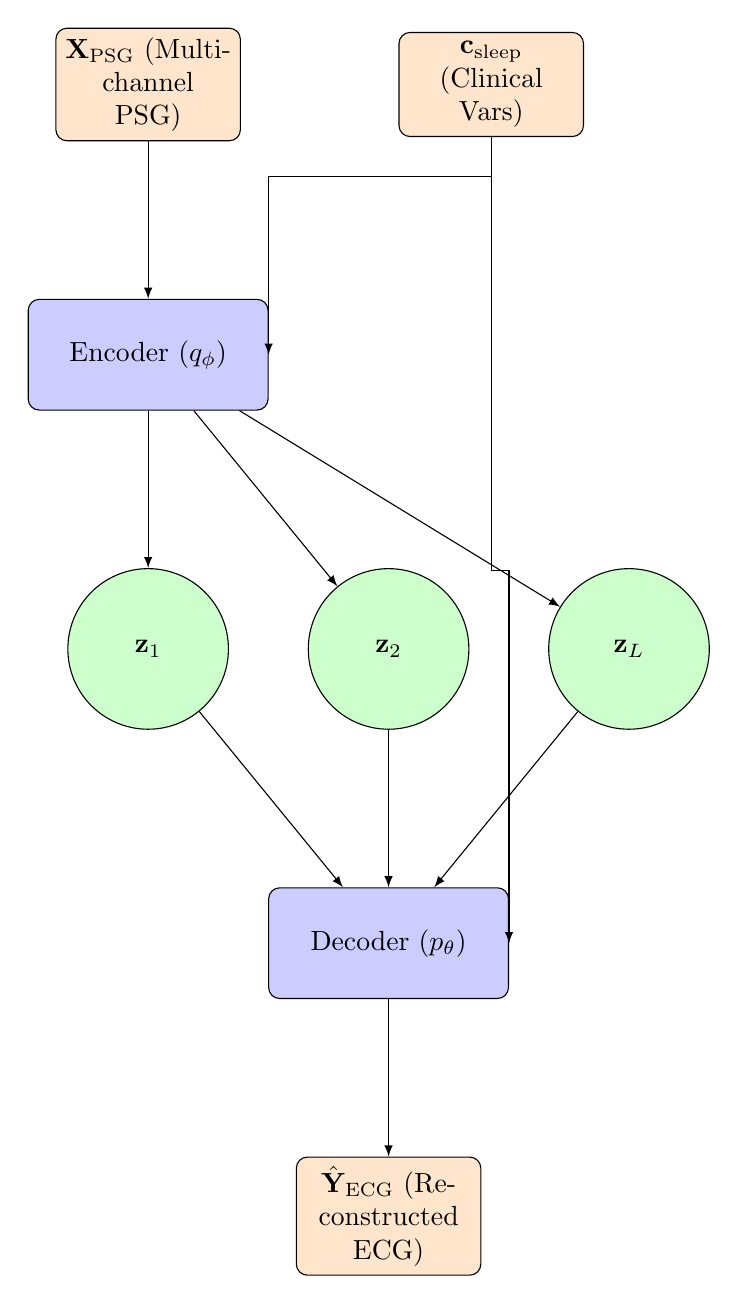
\begin{tikzpicture} [
        auto,
        block/.style={rectangle, draw, fill=blue!20, text width=8em, text centered, rounded corners, minimum height=4em},
        latent/.style={circle, draw, fill=green!20, text width=5em, text centered, minimum height=3em},
        io/.style={rectangle, draw, fill=orange!20, text width=6em, text centered, rounded corners, minimum height=3em},
        line/.style={draw, -latex}
    ]
        % Nodes
        \node[io] (psg) {$\mathbf{X}_{\text{PSG}}$ (Multi-channel PSG)};
        \node[io, right=2cm of psg] (clinical) {$\mathbf{c}_{\text{sleep}}$ (Clinical Vars)};
        
        \node[block, below=2cm of psg] (encoder) {Encoder ($q_\phi$)};
        
        \node[latent, below=2cm of encoder] (z1) {$\mathbf{z}_1$};
        \node[latent, right=1cm of z1] (z2) {$\mathbf{z}_2$};
        \node[coordinate, right=0.5cm of z2] (dots) {};
        \node[latent, right=0.5cm of dots] (zL) {$\mathbf{z}_L$};
        
        \node[block, below=2cm of z2] (decoder) {Decoder ($p_\theta$)};
        
        \node[io, below=2cm of decoder] (ecg) {$\hat{\mathbf{Y}}_{\text{ECG}}$ (Reconstructed ECG)};

        % Paths
        \path [line] (psg) -- (encoder);
        \path [line] (clinical.south) -- ++(0,-0.5) -| (encoder.east);
        \path [line] (encoder) -- (z1);
        \path [line] (encoder) -- (z2);
        \path [line] (encoder) -- (zL);
        
        \path [line] (z1) -- (decoder);
        \path [line] (z2) -- (decoder);
        \path [line] (zL) -- (decoder);
        
        \path [line] (clinical.south) -- ++(0,-5.5) -| (decoder.east);
        
        \path [line] (decoder) -- (ecg);
    \end{tikzpicture}
    \caption{High-level architecture of the cNVAE-PSG model, illustrating the flow from multi-channel PSG and clinical variables to the reconstructed ECG signal through a hierarchical latent space. The encoder $q_\phi$ maps inputs to the latent variables $\mathbf{z}_l$, and the decoder $p_\theta$ reconstructs the ECG, both conditioned on clinical sleep variables $\mathbf{c}_{\text{sleep}}$.}
    \label{fig:cnvae_architecture}
\end{figure}

\printbibliography[heading=bibintoc, title=\ebibname]

\appendix
%\appendixpage
\addappheadtotoc

\section{Derivation of the Conditional VAE Objective}
\label{app:elbo_derivation}

The goal of the cNVAE-PSG is to model the conditional distribution $p(\mathbf{Y}_{\text{ECG}} | \mathbf{X}_{\text{PSG}}, \mathbf{c}_{\text{sleep}})$. We introduce a set of hierarchical latent variables $\mathbf{z} = \{\mathbf{z}_1, \dots, \mathbf{z}_L\}$ to make this modeling tractable. The log-likelihood of observing the ECG data given the PSG and clinical conditions can be written as:
\begin{align}
\log p_\theta(\mathbf{Y}_{\text{ECG}} | \mathbf{X}_{\text{PSG}}, \mathbf{c}_{\text{sleep}}) = \log \int p_\theta(\mathbf{Y}_{\text{ECG}}, \mathbf{z} | \mathbf{X}_{\text{PSG}}, \mathbf{c}_{\text{sleep}}) d\mathbf{z}
\end{align}
Directly optimizing this is intractable due to the integral over $\mathbf{z}$. We introduce an approximate posterior (encoder) $q_\phi(\mathbf{z} | \mathbf{Y}_{\text{ECG}}, \mathbf{X}_{\text{PSG}}, \mathbf{c}_{\text{sleep}})$ to approximate the true posterior $p_\theta(\mathbf{z} | \mathbf{Y}_{\text{ECG}}, \mathbf{X}_{\text{PSG}}, \mathbf{c}_{\text{sleep}})$.

We can then derive the Evidence Lower Bound (ELBO):
\begin{align}
\log p_\theta(\mathbf{Y} | \mathbf{X}, \mathbf{c}) &= \log \int p_\theta(\mathbf{Y}, \mathbf{z} | \mathbf{X}, \mathbf{c}) d\mathbf{z} \\
&= \log \int q_\phi(\mathbf{z} | \mathbf{Y}, \mathbf{X}, \mathbf{c}) \frac{p_\theta(\mathbf{Y}, \mathbf{z} | \mathbf{X}, \mathbf{c})}{q_\phi(\mathbf{z} | \mathbf{Y}, \mathbf{X}, \mathbf{c})} d\mathbf{z} \\
&\geq \int q_\phi(\mathbf{z} | \mathbf{Y}, \mathbf{X}, \mathbf{c}) \log \frac{p_\theta(\mathbf{Y}, \mathbf{z} | \mathbf{X}, \mathbf{c})}{q_\phi(\mathbf{z} | \mathbf{Y}, \mathbf{X}, \mathbf{c})} d\mathbf{z} \quad (\text{Jensen's Inequality}) \\
&= \mathbb{E}_{q_\phi(\mathbf{z}|\mathbf{Y},\mathbf{X},\mathbf{c})} \left[ \log p_\theta(\mathbf{Y}, \mathbf{z} | \mathbf{X}, \mathbf{c}) - \log q_\phi(\mathbf{z} | \mathbf{Y}, \mathbf{X}, \mathbf{c}) \right] \\
&= \mathbb{E}_{q_\phi} \left[ \log p_\theta(\mathbf{Y} | \mathbf{z}, \mathbf{X}, \mathbf{c}) + \log p_\theta(\mathbf{z} | \mathbf{X}, \mathbf{c}) - \log q_\phi(\mathbf{z} | \mathbf{Y}, \mathbf{X}, \mathbf{c}) \right] \\
&= \underbrace{\mathbb{E}_{q_\phi}[\log p_\theta(\mathbf{Y} | \mathbf{z}, \mathbf{X}, \mathbf{c})]}_{\text{Reconstruction Term}} - \underbrace{\KL{q_\phi(\mathbf{z} | \mathbf{Y}, \mathbf{X}, \mathbf{c})}{p_\theta(\mathbf{z} | \mathbf{X}, \mathbf{c})}}_{\text{KL Divergence Term}}
\end{align}
For simplicity, we denote $\mathbf{Y} = \mathbf{Y}_{\text{ECG}}$, $\mathbf{X} = \mathbf{X}_{\text{PSG}}$, and $\mathbf{c} = \mathbf{c}_{\text{sleep}}$. The objective is to maximize this ELBO, which is equivalent to minimizing its negative, $\mathcal{L}_{\text{ELBO}}$. This forms the basis of our loss function, combining the reconstruction loss and the KL divergence regularization term.

\section{Interpretation of Hierarchical Latent Scales}
\label{app:latent_scales}

The multi-scale latent hierarchy is designed to disentangle physiological processes occurring at different timescales during sleep. Table \ref{tab:latent_interpretation} details the intended role of each scale.

\begin{table}[ht]
\centering
\caption{Physiological Interpretation of Latent Variable Scales}
\label{tab:latent_interpretation}
\begin{tabular}{llll}
  \toprule
  \textbf{Scale} & \textbf{Window Size} & \textbf{Primary Physiological Target} & \textbf{Electrophysiological Features Encoded} \\
  \midrule
  $z_1$ & $\sim$15 sec & Beat-to-beat dynamics and fast respiratory coupling & QRS morphology, QT interval, P-wave presence, immediate heart rate response to respiratory phase (Respiratory Sinus Arrhythmia). \\
  $z_2$ & $\sim$30 sec & Short-term autonomic regulation and sleep microarchitecture & Heart rate variability (e.g., RMSSD), response to arousals, patterns associated with specific respiratory events (apneas, hypopneas). \\
  $z_3$ & $\geq$60 sec & Sleep macroarchitecture and circadian influence & Overall autonomic state (sympathetic vs. parasympathetic dominance), sleep stage characteristics (e.g., stable HR in N3 vs. variable HR in REM), long-term HR trends. \\
  \bottomrule
\end{tabular}
\end{table}

\end{document}
